\section{Introduction}


Large language model (LLM) alignment via reinforcement learning (RL) has achieved substantial progress, where a policy model's parameters are iteratively updated to maximize rewards from an oracle~\citep{ppo, ouyangrlhf, grpo}. The effectiveness of this process hinges on the quality of the reward function. However, a core challenge arises when training LLMs on heterogeneous tasks: a single, generic reward model often lacks the discriminative power for specific domains due to distribution shifts. Meanwhile, creating specialized reward models for each task is frequently impractical, facing obstacles like catastrophic forgetting, the need for expert domain knowledge for data annotation, and prohibitive costs.

This situation highlights a crucial gap and a significant opportunity. The open-source community has developed numerous high-quality, task-specific reward models~\citep{skyworkreward, cai2024internlm2, yang2024gpt2helpful, nicholas22rewardreward, seedX, tulu3}, available on platforms like \textit{HuggingFace} and \textit{ModelScope}\footnote{\url{https://huggingface.co/}, \url{https://modelscope.cn/}}. These specialized models typically outperform generic evaluators on their intended tasks, yet remain an underutilized resource. We argue for a paradigm shift: instead of training new static models that directly output sample-specific rewards, a more scalable and cost-effective approach is to orchestrate these existing assets as reward functions that compute rewards for each sample with the corresponding distribution expertise when correctly assigned.

\begin{wrapfigure}{r}{0.5\textwidth}
    \centering
    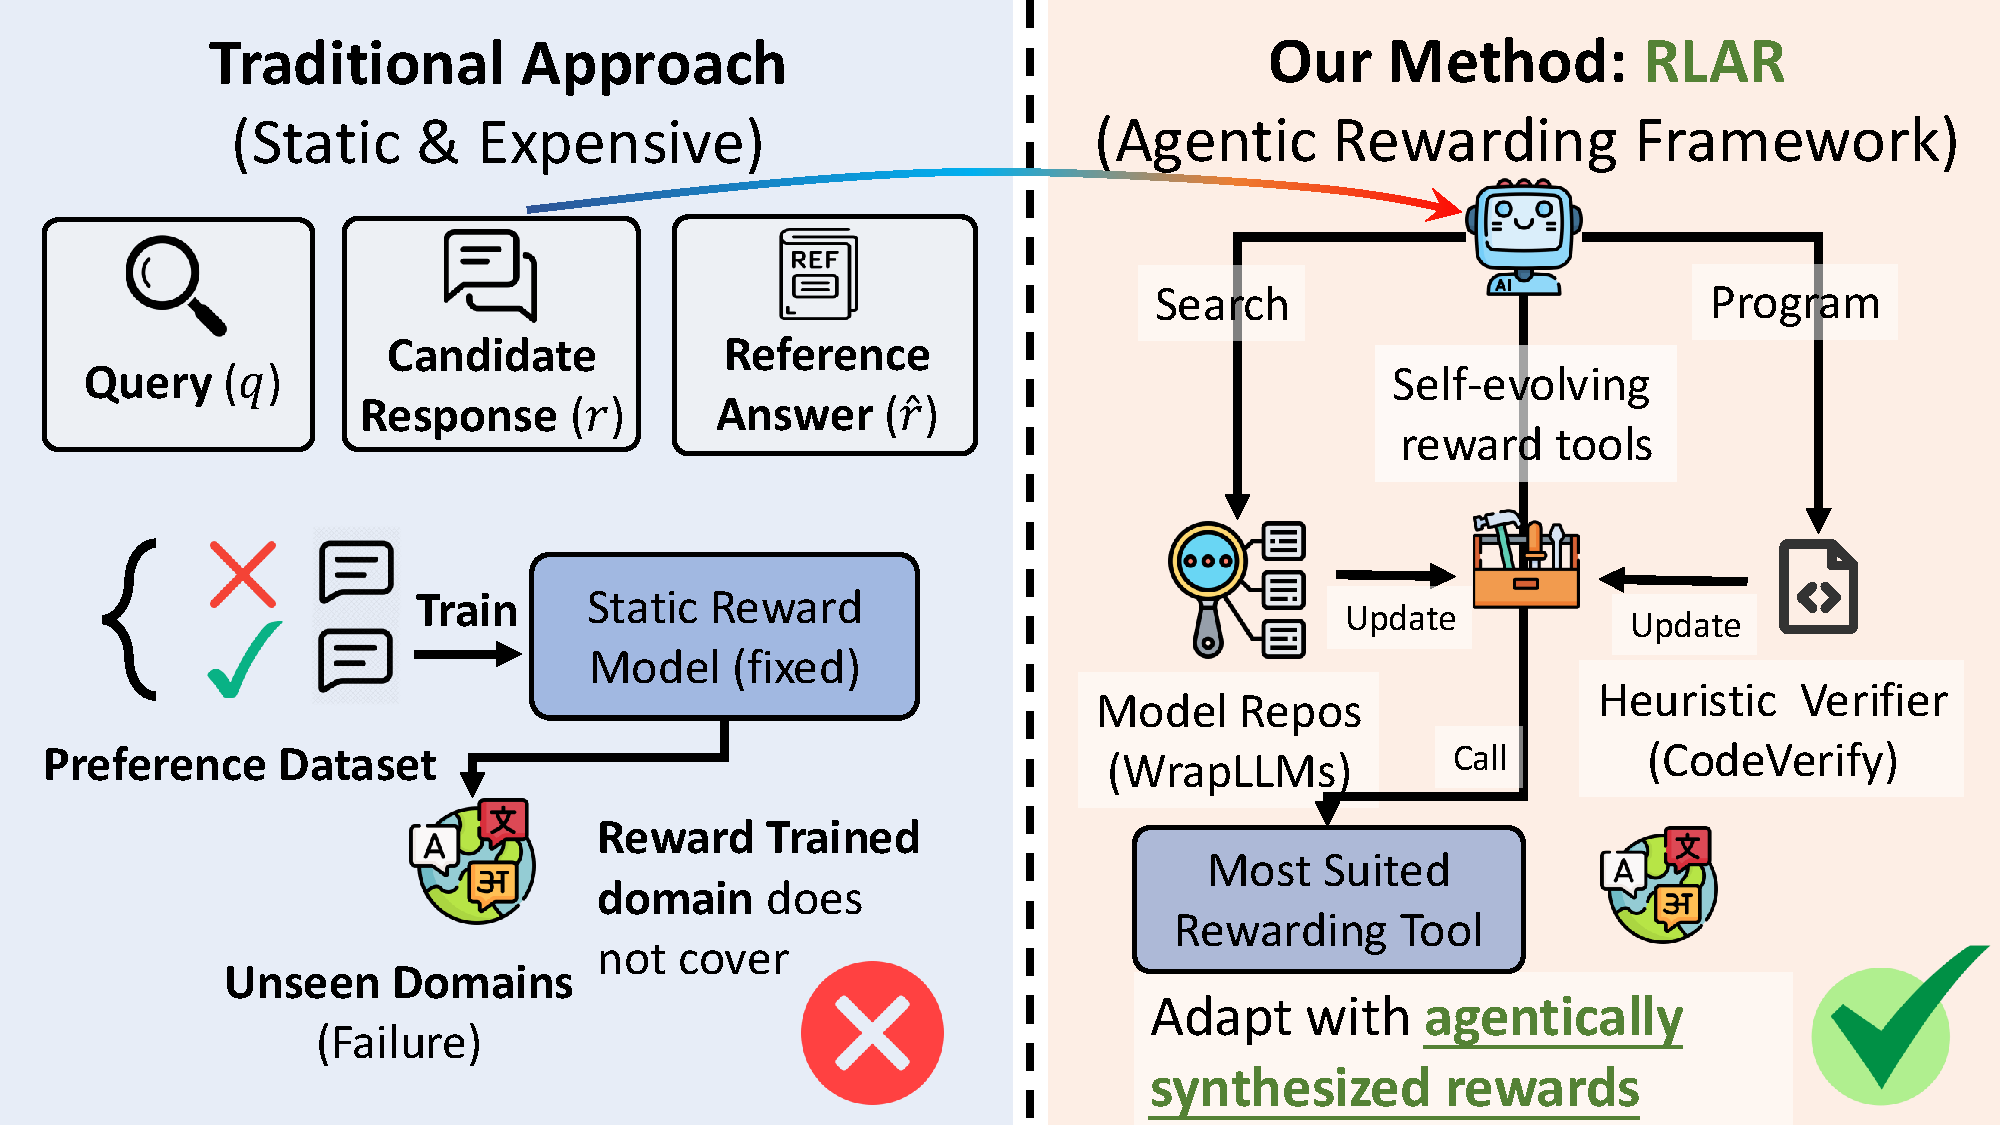
\includegraphics[width=0.95\linewidth]{Figures/intro_fig.pdf}
    \caption{A conceptual comparison between traditional reward modeling and our proposed RLAR framework.}
    \label{fig:intro_fig}
    \vspace{-4mm}
\end{wrapfigure}

To bridge this gap, we propose \textbf{\method{}} (Reinforcement Learning from Agentic Rewards), a self-evolving framework that \textbf{regards the reward functions as callable tools} and is easy to scale over heterogeneous query distributions.
\method{} primarily leverages LLMs' tool-calling capabilities to assign reward scores for the querying task sample based on existing tools. 
Once there are no suitable local tools, \method{} explores online model checkpoint repositories in search of matching neural models, as well as designs code-based executable functions for the current task. The runtime tool library evolves with the appended tools.
We calibrate the final reward output from \method{} with benchmarks such as \textsc{RewardBench-V2}~\citep{rewardbench2} before deploying it in online RL training.
By shifting from learning LLMs' ``\textbf{generated score reward}'' to ``\textbf{designed reward function}'', \method{} ensures high-fidelity rewards across distributions while significantly reducing the inference costs associated with constructing additional reward models.

We evaluate \method{} across a diverse suite of tasks, including math reasoning~\citep{hendrycks2021measuringmathematicalproblemsolving, gsm8k}, code~\citep{leetcodedataset, mbpp}, translation~\citep{benchmax, nllb2022, flores101, twoevaldatasets}, and general chat~\citep{ultrachat}.
We compare our agentic reward synthesis-leveraging framework against state-of-the-art static reward models, including classification~\citep{skyworkreward}, generative ones~\citep{skyworkcritic2024}, and GPT5-as-a-judge. 
\method{} achieves overall performance improvements of \(10.4\%\) and \(61.9\%\) on Llama-3.1-8B and Qwen3-8B, significantly surpassing static classification and generative baselines. 
Unlike baselines such as \textbf{SkyLlama}, which suffer from performance decrements in math reasoning tasks during mixed training, \method{} dynamically models domain objectives across math, code, translation, and chat. 
Notably, \method{} demonstrates enhanced robustness to \textbf{format and verbosity hacking}, whereas loopholes persist in baselines, including GPT5-as-a-judge.
Finally, compared to GPT-5-as-a-judge, \method{} reduces API token consumption by approximately \(80\%\) and GPU training hours by \(75\%\), demonstrating \method{}'s scaling potential.
Ablation studies reveal that each synthesis pathway serves a distinct role: \textbf{CodeVerify}-generated verifiers are critical for rule-heavy tasks (math, code), while \textbf{WrapLLM}-retrieved neural models are essential for open-ended tasks (chat, translation). Furthermore, replacing the agentic selector with random reward assignment degrades performance across nearly all benchmarks, confirming that \method{}'s gains stem from precise per-query reward routing, not merely from reward tool diversity.
The data and code are available on \url{https://anonymous.4open.science/r/NeurIPS2026-RLAR/}.


% Further experiments demonstrate that the effectiveness of RLAR mainly comes from the accurate reward tool selection, and we calibrate it with \textsc{RewardBench-v2}. Our \textbf{Agentic Reward Tool Selector} obtained \(90.44\%\) accuracy by routing queries to the most suitable reward models, outperforming both the SOTA \(87.19\%\) and SOTA-model logits ensembling \(87.44\%\). These results indicate that dynamic routing more effectively approaches the theoretical upper bound. 

